\documentclass[11pt,a4paper]{article}

\usepackage[margin=1in]{geometry}
\usepackage{amsmath,amssymb,bm}
\usepackage{graphicx}
\usepackage{booktabs}
\usepackage{enumitem}
\usepackage[hidelinks]{hyperref}
\usepackage{setspace}
\onehalfspacing

\graphicspath{{figures/}}

\title{Procedure and Methods:\\
Sedov--Taylor + Gauss decreasing-density model\\
and Migkas angular comparison}
\author{Working notes (Cosmology project)\\
\textit{Not a submitted methods section --- living draft}}
\date{18 September 2026}

\begin{document}
\maketitle

\noindent
This document records the \textbf{ordered steps} of the model setup and calculations used in the present program: geometry, homologous expansion, Gauss gravity with decreasing density, spreadsheet / numerical evaluation, phase (axis) rotation, and comparison to Migkas et~al.\ (2020) Fig.~6 longitude strips with uncertainties.

\section{Scientific target and ontology}

\begin{enumerate}[leftmargin=*]
\item \textbf{Observational target.} Migkas et~al.\ (2020) Fig.~6: best-fit \(L_X\)--\(T\) normalization \(A/A_{\mathrm{all}}\) and slope \(B/B_{\mathrm{all}}\) versus Galactic longitude \(\ell\) in scanning strips of width \(\Delta\ell=90^\circ\) (full latitude), with uncertainties.
\item \textbf{Ontology (binding).} The Universe has a real geometric center of expansion (CoE) beyond the observable horizon. The observer sits off-center at Euclidean distance \(D\) from the CoE. The goal is to challenge the cosmological principle with a first-principles centered model, not to fit a free dipole template \(A\cos\phi\) inside \(\Lambda\)CDM.
\item \textbf{Success criterion for the angular diagnostic.} After a simple sky-axis / phase alignment, the model longitude series should track \emph{both} Migkas \(A\) and \(B\) bars (sheet diagnostic: \(R^2\sim 0.74\) for each). Separately, a pure ST+Gauss \(H_{\mathrm{obs}}\) map must eventually pass a Migkas-like \(\theta\simeq 75^\circ\) cone-scan filter (open).
\end{enumerate}

\section{Step 1 --- Geometry}

\begin{enumerate}[leftmargin=*]
\item Place the CoE at the origin.
\item Place the observer at \(\vec{D}\) with \(D=\|\vec{D}\|\) and unit vector \(\hat{D}=\vec{D}/D\) (CoE \(\to\) observer).
\item Place a source at \(\vec{r}\) (CoE-radius \(r=\|\vec{r}\|\)).
\item Define the observer--source separation
\[
\vec{d}=\vec{r}-\vec{D},\qquad d=\|\vec{d}\|,\qquad \hat{n}=\vec{d}/d.
\]
\item On the spreadsheet / toy sky, sample sources on a circle of fixed observer-centric radius \(R\) about the observer:
\[
\vec{r}=\vec{D}+R\,(\cos\varphi,\sin\varphi),
\]
with Earth-centric angle \(\varphi\) measured from \(+\hat{D}\) (so \(\varphi=0\) is anti-center, \(\varphi=\pi\) toward the CoE). Tabulate \(\varphi=0^\circ,1^\circ,\ldots,359^\circ\) (or equivalent).
\item Record Cartesian components \(P_x,P_y\), then \(r=\|\vec{r}\|\) and \(d=R\) on that circle.
\end{enumerate}

\begin{figure}[ht]
\centering
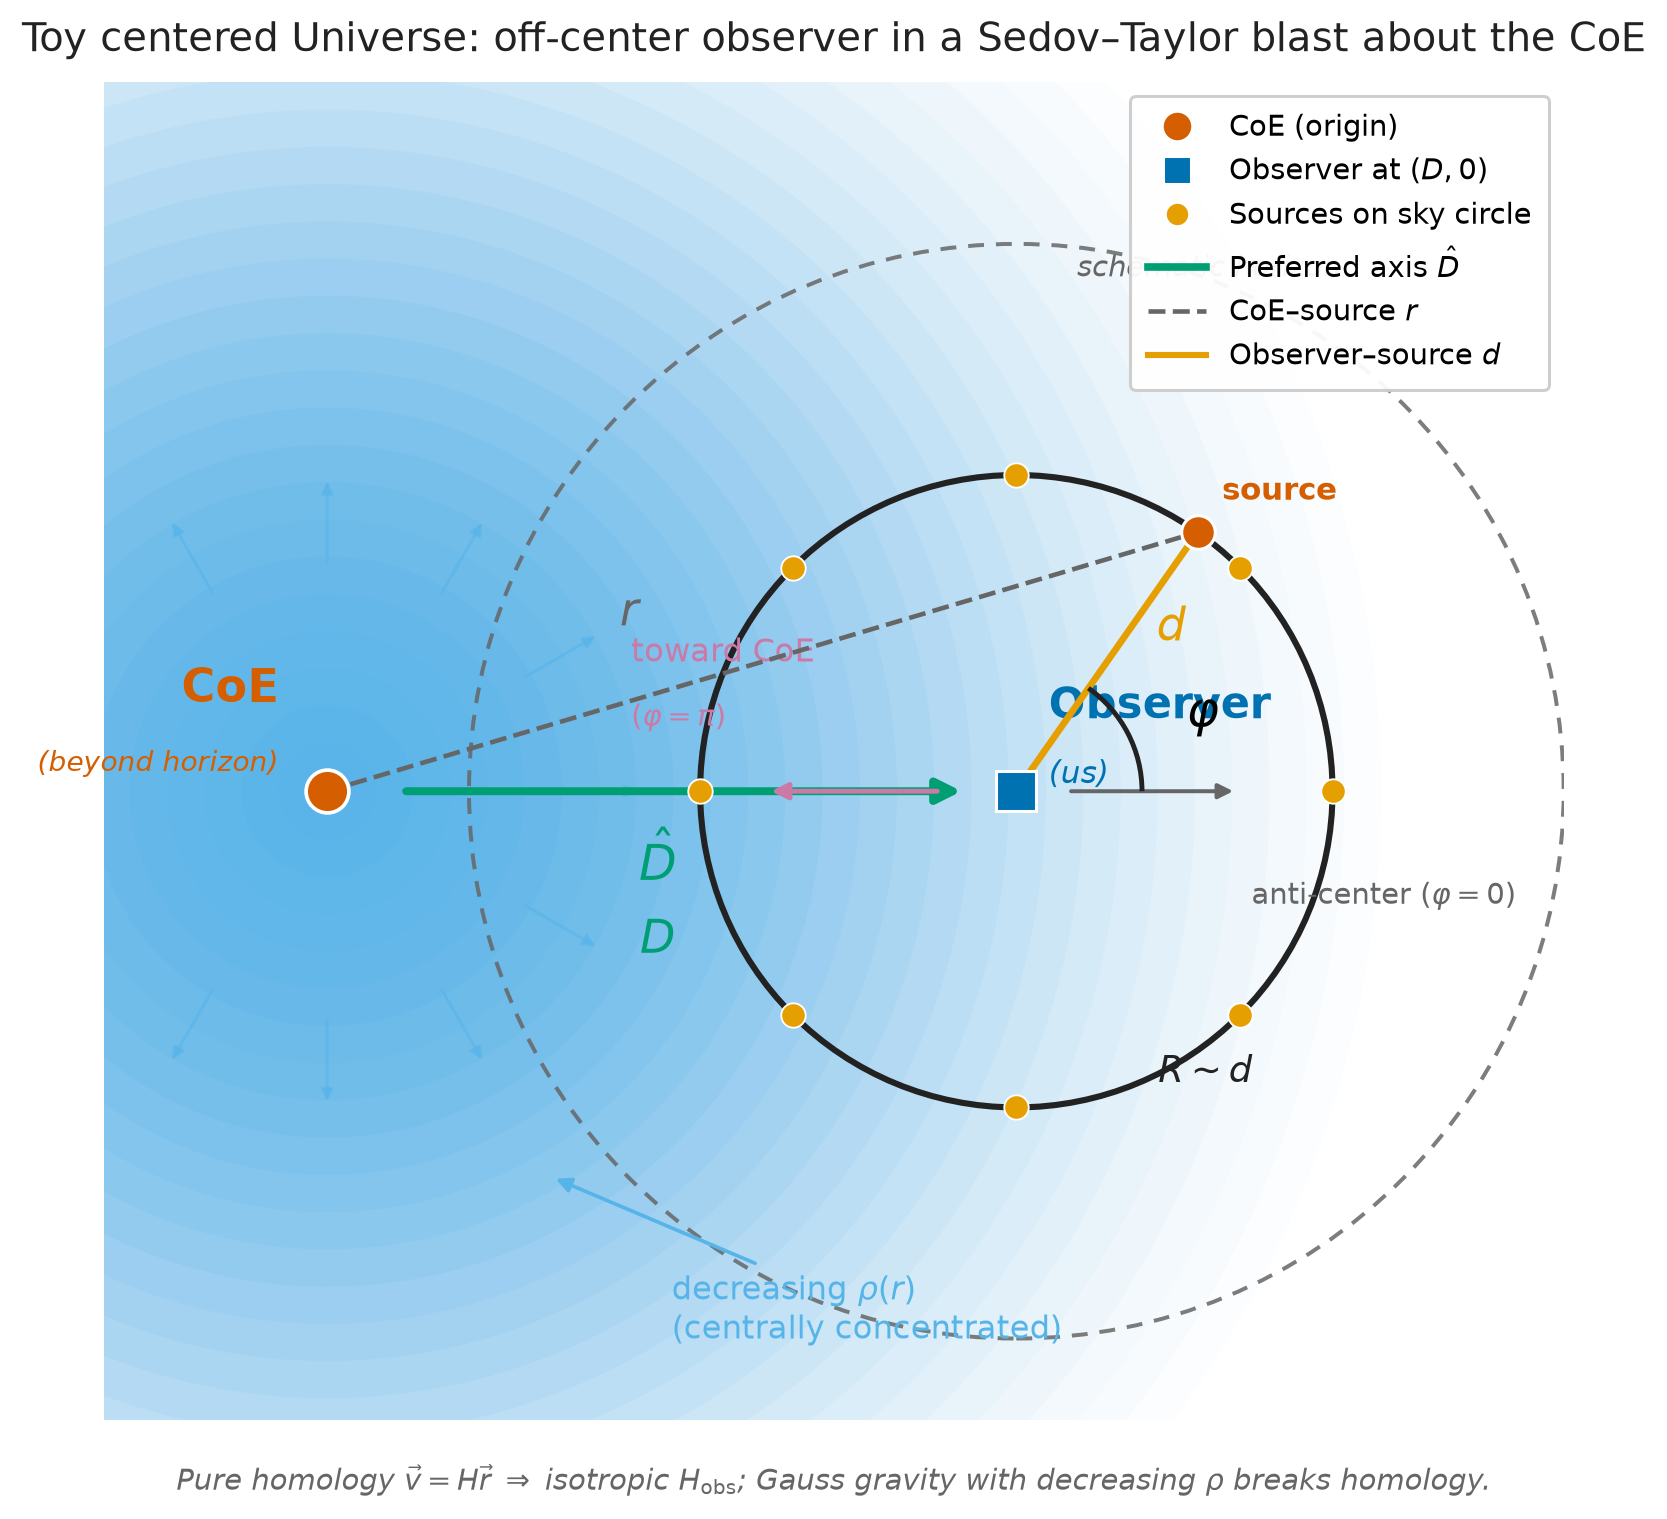
\includegraphics[width=0.82\linewidth]{geometry.png}
\caption{Geometry used in Steps~1--4: CoE, observer at \(D\), source at \(r\), separation \(d\), Earth-centric angle \(\varphi\).}
\end{figure}

\section{Step 2 --- Sedov--Taylor homologous background}

\begin{enumerate}[leftmargin=*]
\item Adopt a Sedov--Taylor (ST) blast-wave analogy with Hubble-like rate
\[
H(t)\equiv \frac{\dot{R}_{\mathrm{ST}}}{R_{\mathrm{ST}}}.
\]
(Cosmological map of blast energy and ambient density is left undefined; \(H\) is treated as an input scale.)
\item Interior homology (working assumption):
\[
\vec{v}(\vec{r},t)=H(t)\,\vec{r}.
\]
\item Observer velocity \(\vec{v}_O=H\vec{D}\); source velocity \(\vec{v}_S=H\vec{r}\).
\item Relative recession (must subtract observer motion):
\[
\vec{v}_{\mathrm{rel}}=H\vec{d},\qquad
v_{\mathrm{los}}=\vec{v}_{\mathrm{rel}}\cdot\hat{n}=H\,d,\qquad
H_{\mathrm{obs}}=\frac{v_{\mathrm{los}}}{d}=H.
\]
\item \textbf{Homology theorem (mandatory check).} For pure ST, \(H_{\mathrm{obs}}=H\) is independent of direction for any \(D\). If a numerical run shows angular variation at \(M=0\), the code failed to subtract \(\vec{v}_O\) (frame error) and must be fixed before gravity is added.
\end{enumerate}

\section{Step 3 --- Decreasing density and Gauss gravity}

\begin{enumerate}[leftmargin=*]
\item Reject uniform density: \(M(<r)\propto r^3\Rightarrow g\propto -r\) yields only a monopole in \(H_{\mathrm{obs}}\) after differencing.
\item Adopt a centrally concentrated decreasing density whose cumulative mass is the incomplete-gamma form used in the spreadsheet (Phase~A eq.~3.13):
\[
\frac{m(r)}{M_{\mathrm{tot}}}
=1-e^{-X}\Bigl(1+X+\frac{X^2}{2}\Bigr),
\qquad X=\frac{r}{L},
\]
corresponding to \(\rho(r)\propto e^{-r/L}\). Here \(L\) (sheet ``density length'') sets the concentration; binding runs use \(D/L\sim\mathcal{O}(5\)--\(7)\).
\item Enclosed mass toward the CoE at the observer:
\[
M_{\mathrm{enc}}\equiv m(D).
\]
In the sheet, the labeled mass parameter is tied to \(M_{\mathrm{enc}}\) (or to \(M_{\mathrm{tot}}\) via the cumulative fraction); keep the identification explicit when changing units.
\item Gauss acceleration at CoE-radius \(r\):
\[
\vec{g}(r)=-\frac{G\,m(r)}{r^2}\,\hat{r}.
\]
\item Peculiar-velocity ansatz (placeholder until full time integration from the blast):
\[
\vec{u}(r)=-\alpha\,\frac{G\,m(r)}{r^2 H}\,\hat{r},
\qquad \alpha\sim\mathcal{O}(1).
\]
(Intended physics: integrate \(\vec{g}\) from the initial blast forward in time; the \(\alpha/H\) form is the instantaneous O(1) surrogate.)
\item Relative LOS velocity with gravity:
\[
\vec{v}_{\mathrm{rel}}=H\vec{d}+\bigl[\vec{u}(\vec{r})-\vec{u}(\vec{D})\bigr],
\qquad
H_{\mathrm{obs}}(\hat{n},d)=H+\frac{\delta v}{d}.
\]
\item Natural dimensionless amplitude (binding):
\[
\kappa\equiv\frac{G M_{\mathrm{enc}}}{D^3 H^2}
=\frac{\Omega_m}{2}\approx 0.15
\quad(\Omega_m=0.3).
\]
This equates the mean enclosed density \(\bar\rho(<D)=3M_{\mathrm{enc}}/(4\pi D^3)\) with \(\Omega_m\rho_{\mathrm{crit}}\) up to the factor that makes \(\kappa=\Omega_m/2\). Local \(\rho(D)\) in the exponential tail is \emph{lower} than \(\bar\rho(<D)\) (typically by \(\sim 10\)--\(15\times\) at \(D/L\sim 6.7\)); that is intentional for a decreasing profile, not a bug in \(\kappa\).
\end{enumerate}

\begin{figure}[ht]
\centering
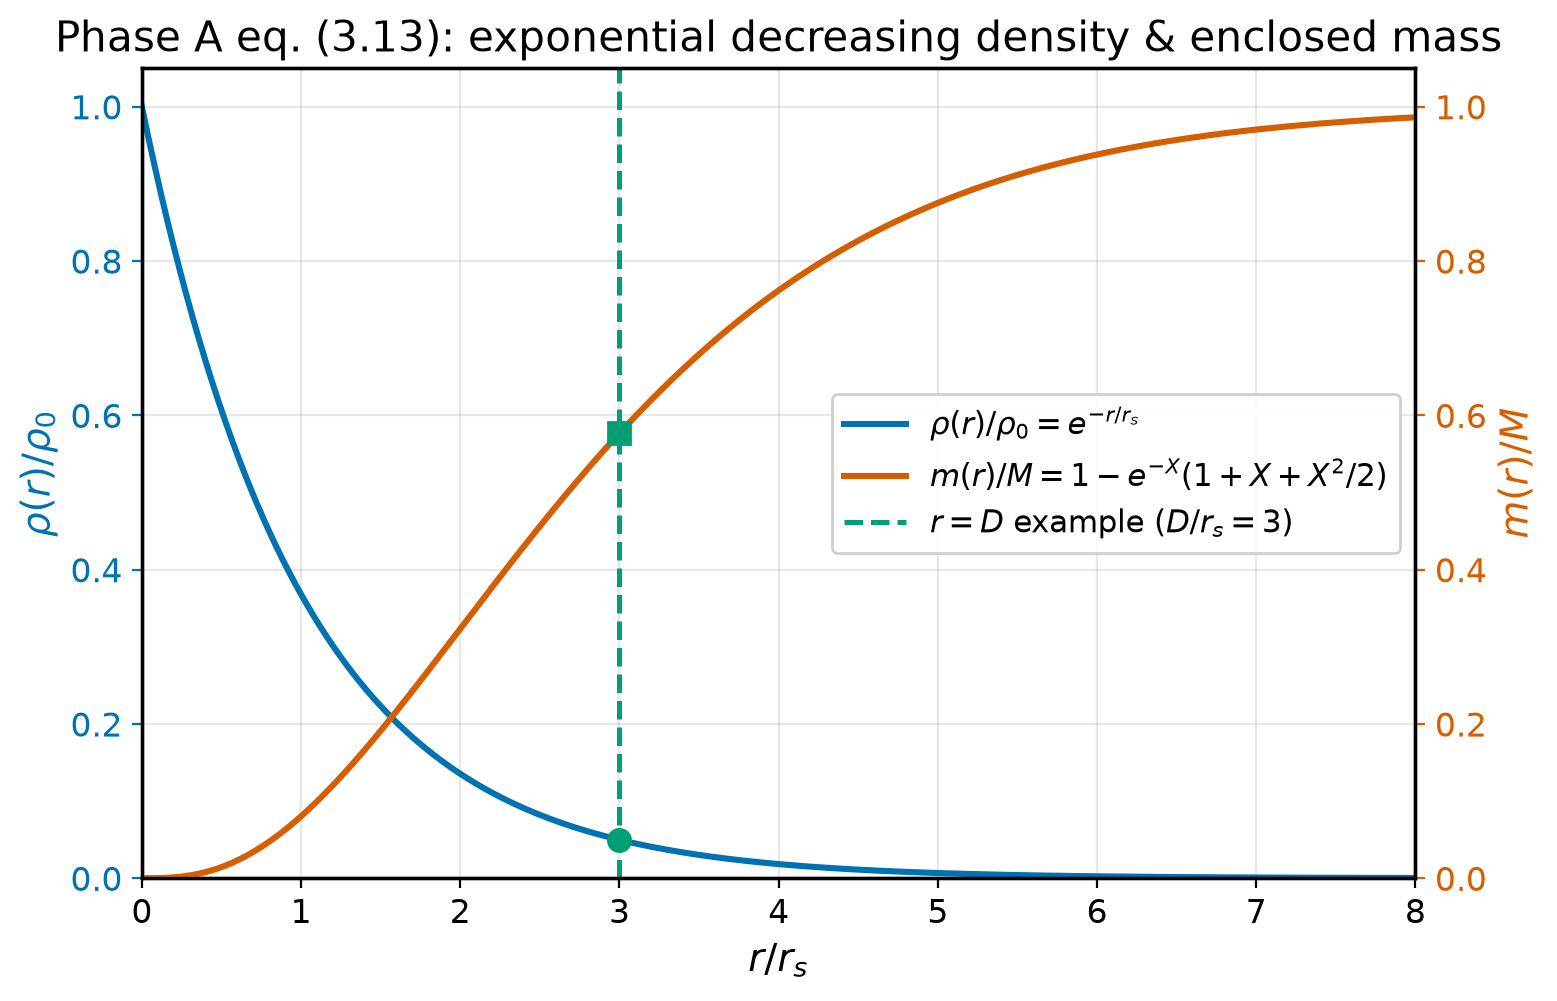
\includegraphics[width=0.85\linewidth]{density_mass.png}
\caption{Illustrative decreasing \(\rho(r)\) and cumulative \(M(<r)\) used in Step~3.}
\end{figure}

\section{Step 4 --- Numerical evaluation on the sky circle}

For each angle \(\varphi\) on the observer-centered circle of radius \(R\):

\begin{enumerate}[leftmargin=*]
\item Compute \(\vec{r}\), \(r\), \(m(r)\), \(\vec{g}\) or \(\vec{u}\) at the source and at the observer.
\item Form ST velocities \(\vec{v}_S=H\vec{r}\), \(\vec{v}_O=H\vec{D}\) and peculiar difference \(\vec{u}(\vec{r})-\vec{u}(\vec{D})\).
\item Project onto \(\hat{n}\) to obtain \(v_{\mathrm{los}}\) and
\[
\frac{H_{\mathrm{obs}}}{H}=\frac{v_{\mathrm{los}}}{H\,d}.
\]
\item Store the series \(H_{\mathrm{obs}}(\varphi)/H\) (sheet column historically tied to recession with acceleration over recession without).
\item Optional: map to an \(A\)-like quantity via luminosity-distance / flux scaling, e.g.\ \(A\propto H^{-2}\),
\[
\frac{A}{A_{\mathrm{all}}}\propto\frac{1}{(H_{\mathrm{obs}}/H)^2},
\]
renormalised to mean unity over \(\varphi\) when comparing to Migkas \(A/A_{\mathrm{all}}\).
\end{enumerate}

\noindent
\textbf{Binding baseline parameters (unitless spreadsheet).} Typical working set: \(H\equiv k=1\), \(G=1\), \(D\sim 10\), \(R\sim 2\)--\(3\), \(L\sim 1.5\), \(M_{\mathrm{enc}}\) chosen so \(\kappa\sim 0.05\)--\(0.15\). Physical-unit copy tabs exist but are not trusted until \(G\), \(H\), and \(M\) are mutually consistent with \(\kappa\sim\Omega_m/2\).

\section{Step 5 --- Migkas data: digitise Fig.~6 bars}

\begin{enumerate}[leftmargin=*]
\item Obtain Migkas et~al.\ (2020) Fig.~6 (top \(A/A_{\mathrm{all}}\), bottom \(B/B_{\mathrm{all}}\) vs Galactic longitude).
\item Digitise central values and asymmetric error bars on the \(\Delta\ell=90^\circ\) strip series.
\item Store as CSV with columns
\[
\ell,\quad A/A_{\mathrm{all}},\quad A_{\mathrm{err}}^{\mathrm{lo}},\quad A_{\mathrm{err}}^{\mathrm{hi}},\quad
B/B_{\mathrm{all}},\quad B_{\mathrm{err}}^{\mathrm{lo}},\quad B_{\mathrm{err}}^{\mathrm{hi}}.
\]
(Present file: \texttt{migkas/fig6\_digitized.csv}, \(\sim 5^\circ\) sampling, 71 points.)
\item Always plot Migkas points \textbf{with error bars} in comparison figures (same presentation as the published figure).
\end{enumerate}

\section{Step 6 --- Phase (axis) rotation diagnostic}

The spreadsheet ``rotation'' is a \textbf{simple sine phase shift} of the angular template (not a 3D geometric re-solve of the CoE for each trial, and not a free dipole MCMC).

\begin{enumerate}[leftmargin=*]
\item Define
\[
S(\ell;\phi)=A_{\mathrm{mp}}\sin\!\Bigl(\frac{2\pi}{360}\,\ell+\phi\Bigr),
\]
with amplitude \(A_{\mathrm{mp}}\) and phase \(\phi\) in radians (sheet: \(\omega=2\pi/360\) so \(\ell\) is in degrees).
\item Binding sheet values (tab \emph{Copy of Copy of Copy of density}):
\[
A_{\mathrm{mp}}=-0.06,\qquad \phi=0.35\ \mathrm{rad}\approx 20.05^\circ.
\]
Opposite amplitude for \(B\): \(B_{\mathrm{mp}}=-A_{\mathrm{mp}}\).
\item Construct rotated model series from the ST columns (sheet notation):
\begin{align*}
\mathrm{Model}_A &= \bigl(1-S_A(\ell;\phi)\bigr)\times(\mathrm{ST\ }A\text{-like series}),\\
\mathrm{Model}_B &= \bigl(1-S_B(\ell;\phi)\bigr)\times(\mathrm{ST\ }B\text{-like series}).
\end{align*}
\item Align model longitudes to Migkas \(\ell\) (sheet: \texttt{VLOOKUP} / interpolation onto the Migkas angle grid).
\item Compute ordinary coefficients of determination \(R^2\) for Migkas vs model, \emph{with} and \emph{without} the sine phase factor. Report the ratio \(R^2_{\mathrm{with}}/R^2_{\mathrm{without}}\) (sheet cells historically \texttt{R2w/R2wo}).
\item Optional: scan shared \(\phi\) to maximise a joint \(A\)+\(B\) score; record best \(\phi\) separately from the author's fixed \(\phi=0.35\).
\end{enumerate}

\noindent
\textbf{Recorded results (18 Sep 2026).}
\begin{center}
\begin{tabular}{@{}lcc@{}}
\toprule
Series & \(R^2\) without rotation & \(R^2\) with sheet rotation \\
\midrule
\(A/A_{\mathrm{all}}\) (sheet 1° grid) & \(0.501\) & \(\mathbf{0.739}\) \\
\(B/B_{\mathrm{all}}\) (sheet 1° grid) & \(0.372\) & \(\mathbf{0.733}\) \\
\(A\) vs digitised CSV+bars & \(0.446\) & \(0.712\) \\
\(B\) vs digitised CSV+bars & \(0.483\) & \(0.785\) \\
\bottomrule
\end{tabular}
\end{center}

\noindent
Best shared-\(\phi\) scan vs digitised bars: \(\phi\approx 0.52\,\mathrm{rad}\) (\(R^2_A\approx 0.730\), \(R^2_B\approx 0.776\)).

\begin{figure}[ht]
\centering
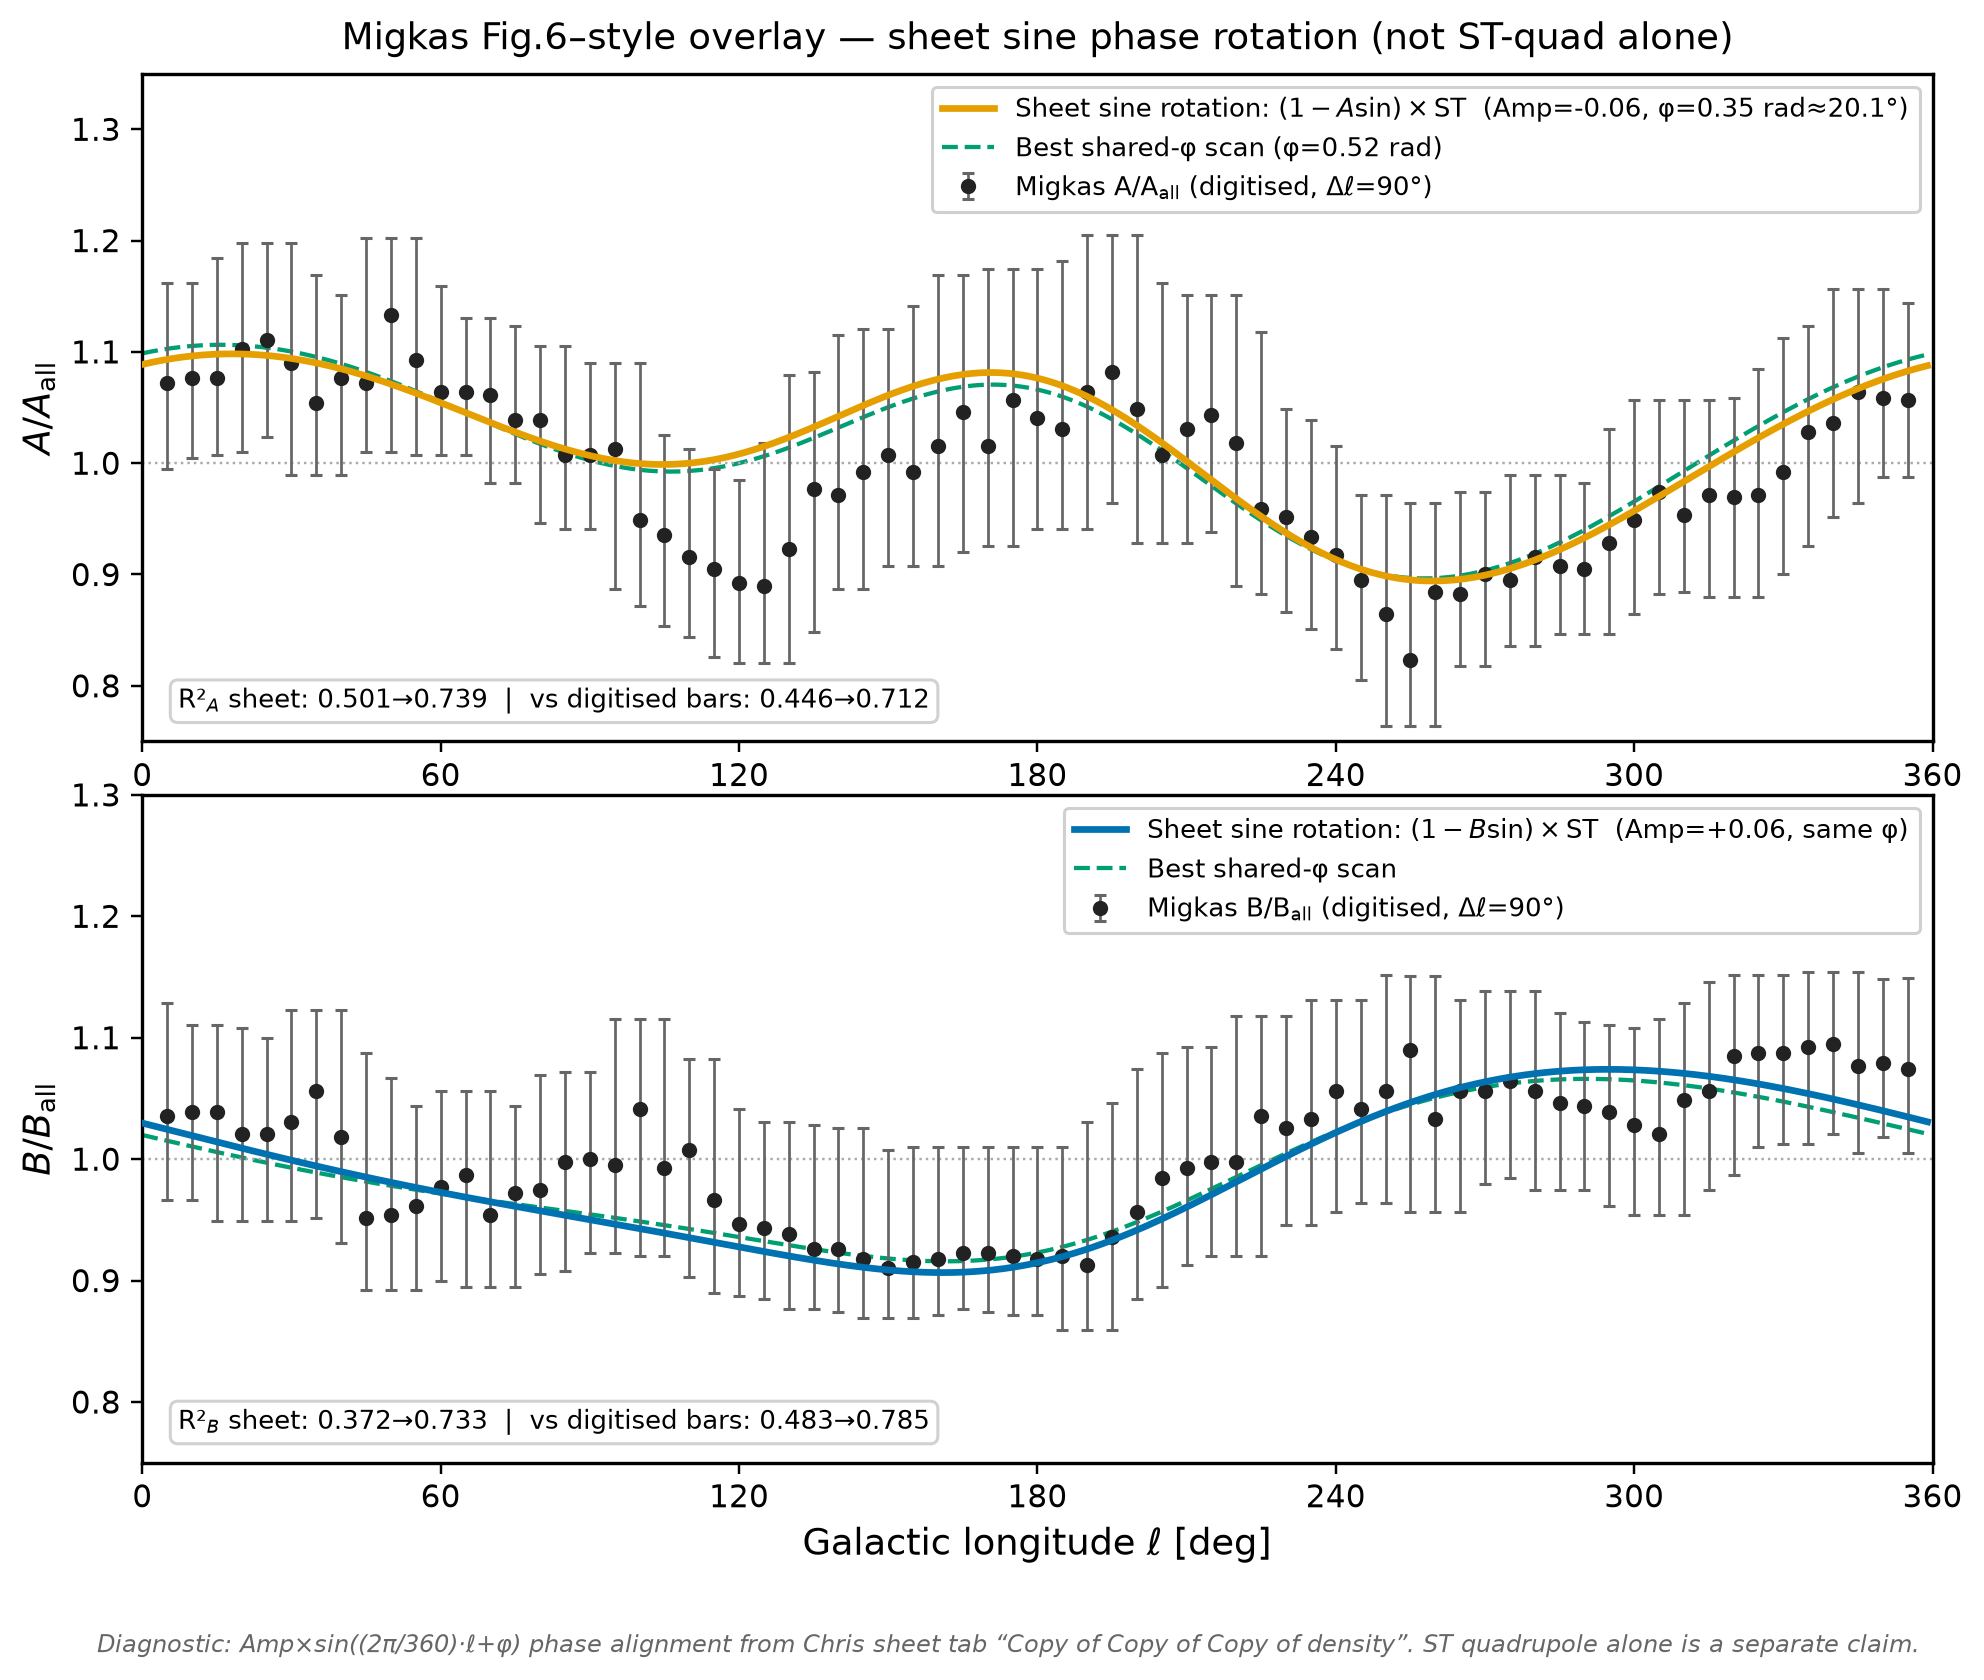
\includegraphics[width=\linewidth]{migkas_bars_rotation_overlay.png}
\caption{Step~6 output: Migkas Fig.~6-style bars for \(A\) and \(B\) with sheet sine-rotation models overlaid.}
\end{figure}

\section{Step 7 --- Fit diagnostics (required plots)}

\begin{enumerate}[leftmargin=*]
\item \textbf{Longitude overlay:} Migkas \(A\) and \(B\) vs \(\ell\) with error bars; model curves after phase rotation on the same axes.
\item \textbf{Scatter:} Migkas vs model for \(A\) and for \(B\), with a plain linear fit \(y=ax+b\) and large \(R^2\).
\item \textbf{Rotation improves fit:} \(R^2\) versus phase \(\phi\) (or sky-axis angle \(\phi_0\)), marking the author's \(\phi\) and any prior related to Migkas's preferred longitude.
\end{enumerate}

\begin{figure}[ht]
\centering
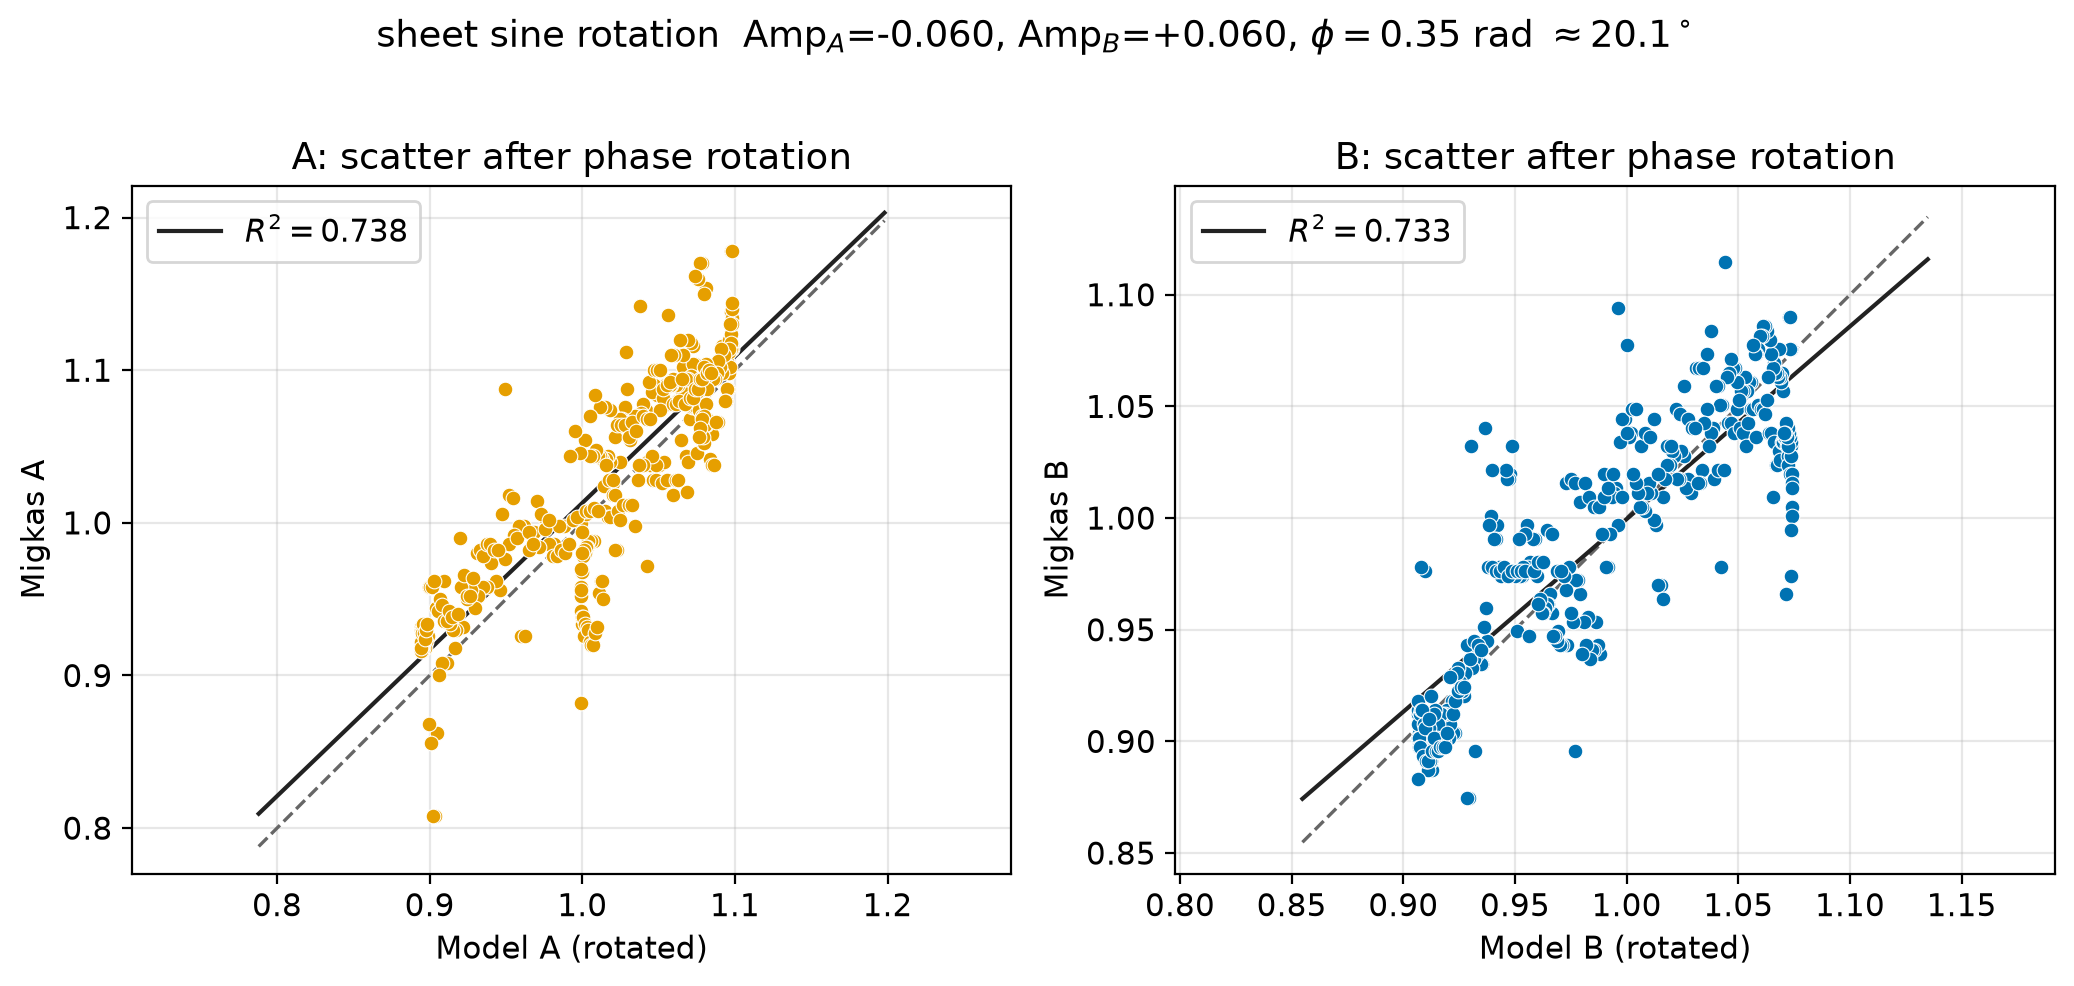
\includegraphics[width=0.95\linewidth]{migkas_bars_rotation_scatter.png}
\caption{Step~7 scatter diagnostics for \(A\) and \(B\) after phase rotation.}
\end{figure}

\section{Step 8 --- Sanity and go / no-go checks}

\begin{enumerate}[leftmargin=*]
\item \(M=0\) (or \(\alpha=0\)): \(H_{\mathrm{obs}}(\varphi)\) must be flat.
\item Uniform \(\rho\): sky anisotropy must collapse relative to decreasing \(\rho\).
\item \(\kappa\) from sheet \((G,M_{\mathrm{enc}},D,H)\) must be \(\mathcal{O}(\Omega_m/2)\); reject unit systems that yield absurd \(\kappa\).
\item Both \(A\) and \(B\) must be shown with Migkas bars; do not report \(B\) as a ``null'' under the sheet rotation diagnostic.
\item Separate claim (weaker until cone-scan exists): raw ST+Gauss quadrupole shape alone vs \(B\) without Amp\(\times\sin\) phase factor.
\end{enumerate}

\section{Step 9 --- Open methods (next, not yet locked)}

\begin{enumerate}[leftmargin=*]
\item Forward-model \(H_{\mathrm{obs}}(\hat{n})\) through Migkas-like \(\theta\simeq 75^\circ\) sky cones / longitude strips (same pipeline as the paper), then retune \(\alpha,\kappa\) only against that filter.
\item Replace the \(\alpha/H\) peculiar ansatz by time-integrated gravity from the blast.
\item Light-travel / luminosity-distance composition (Newtonian \(v_{\mathrm{los}}/d\) is the present pass only).
\item CMB multipole adversary for an off-center observer with a beyond-horizon CoE.
\end{enumerate}

\section{Summary flowchart (calculation order)}

\begin{center}
\renewcommand{\arraystretch}{1.25}
\begin{tabular}{@{}cl@{}}
\toprule
Step & Action \\
\midrule
1 & Fix CoE, \(\vec{D}\), sky circle \((\varphi,R)\) \\
2 & Homologous ST; verify isotropic \(H_{\mathrm{obs}}\) at \(M=0\) \\
3 & Decreasing \(\rho\); Gauss \(g\); \(\kappa=GM_{\mathrm{enc}}/(D^3H^2)\) \\
4 & Compute \(H_{\mathrm{obs}}(\varphi)\); optional \(A\propto H^{-2}\) map \\
5 & Digitise Migkas Fig.~6 \(A,B\) with error bars \\
6 & Apply Amp\(\times\sin(\omega\ell+\phi)\) phase rotation; compute \(R^2\) \\
7 & Overlay, scatter, \(R^2\) vs phase plots \\
8 & Sanity / unit / both-\(A\)-and-\(B\) checks \\
9 & Cone-scan, time-integrated \(g\), light travel, CMB (open) \\
\bottomrule
\end{tabular}
\end{center}

\begin{thebibliography}{9}
\bibitem{Migkas2020}
K.~Migkas et~al., Astron.\ Astrophys.\ \textbf{636}, A15 (2020), arXiv:2004.03305.
\end{thebibliography}

\end{document}
